\documentclass[fleqn,answers,addpoints]{exam}

%\usepackage{graphicx, fancyhdr}
\usepackage{etoolbox}
\usepackage{subcaption}
\usepackage{etoolbox}
\usepackage{tikz,pgfplots}
\usepackage{amsmath, amsfonts}
\usepackage{color}

%% For LaTeX-Box: root = stat105_exam1_info.tex 
%%%%%%%%%%%%%%%%%%%%%%%%%%%%%%%%%%%%%%%%%%%%%%%%%%%%%%%%%%%%%%%%%%%%%%%%%%%%%%%%
%  File Name: stat105_exam1_info.tex
%  Purpose:
%
%  Creation Date: 24-09-2015
%  Last Modified: Thu Sep 24 13:51:36 2015
%  Created By:
%%%%%%%%%%%%%%%%%%%%%%%%%%%%%%%%%%%%%%%%%%%%%%%%%%%%%%%%%%%%%%%%%%%%%%%%%%%%%%%%
\newcommand{\course}[1]{\ifstrempty{#1}{STAT 105}{STAT 105, Section #1}}
\newcommand{\sectionNumber}{B}
\newcommand{\examDate}{October 1, 2015}
\newcommand{\semester}{FALL 2015}
\newcommand{\examNumber}{II}

\newcommand{\examTitle}{Exam \examNumber}

\runningheader{\course{\sectionNumber}}{Exam \examNumber}{\examDate}
\runningfooter{}{}{Page \thepage of \numpages}

\newcommand{\examCoverPage}{
   \begin{coverpages}
   \centering
   {\bfseries\scshape\Huge Exam I \par}
   \vspace{1cm}
   {\bfseries\scshape\LARGE \course{\sectionNumber} \par}
   {\bfseries\scshape\LARGE \semester \par}

   \vspace{2cm}

   \fbox{\fbox{\parbox{5.5in}{\centering 

      \vspace{.25cm} 
      
      {\bfseries\Large Instructions} \\

      \vspace{.5cm} 

      \begin{itemize}
         \item  The exam is scheduled for 80 minutes, from 8:00 to 9:20 AM. At 9:20 AM the exam will end.\\
         \item  A forumula sheet is attached to the end of the exam. Feel free to tear it off.\\
         \item  You may use a calculator during this exam.\\
         \item  Answer the questions in the space provided. If you run out of room, continue on the back of the page. \\
         \item  If you have any questions about, or need clarification on the meaning of an item on this exam, please ask your instructor. No other form of external help is permitted attempting to receive help or provide help to others will be considered cheating.\\
         \item  {\bfseries Do not cheat on this exam.} Academic integrity demands an honest and fair testing environment. Cheating will not be tolerated and will result in an immediate score of 0 on the exam and an incident report will be submitted to the dean's office.\\
      \end{itemize}

   }}}

   \vspace{2cm}

   \makebox[0.6\textwidth]{Name:\enspace\hrulefill}

   \vspace{1cm}

   \makebox[0.6\textwidth]{Student ID:\enspace\hrulefill}
   \end{coverpages}

}


\newcommand{\course}[1]{\ifstrempty{#1}{STAT 305}{STAT 305, Section #1}}
\newcommand{\sectionNumber}{}
\newcommand{\examDate}{May 8, 2019}
\newcommand{\semester}{Spring 2019}
\newcommand{\examNumber}{3}
\newcommand{\qparts}[1]{\begin{parts} #1 \end{parts}}
\newcommand{\qitems}[1]{\begin{itemize} #1 \end{itemize}}

% Document definitions
\newcommand{\examTitle}{Exam \examNumber}
\runningheader{\course{\sectionNumber}}{Exam \examNumber}{\examDate}
\runningfooter{}{}{Page\ \thepage\ of\ \numpages}

\begin{document}

\begin{coverpages}
   \centering
   {\bfseries\scshape\Huge Exam \examNumber \par}
   \vspace{1cm}
   {\bfseries\scshape\LARGE \course{\sectionNumber} \par}
   {\bfseries\scshape\LARGE \semester \par}
   \vspace{2cm}
   \fbox{\fbox{\parbox{5.5in}{
      \centering 
      \vspace{.25cm} 
      {\bfseries\Large Instructions} \\
      \vspace{.25cm} 
      \begin{itemize}
         \item  The exam is scheduled for 120 minutes, from 12:00 to 2:00pm. At  2:00pm  the exam will end.\\
         \item  A forumula sheet is attached to the end of the exam. Feel free to tear it off.\\
         \item  You are allowed to use a self-produced one-page (front and back) formula sheet during this exam.\\
         \item  You may use a calculator during this exam.\\
         \item  Answer the questions in the space provided. If you run out of room, continue on the back of the page. \\
         \item  If you have any questions about, or need clarification on the meaning of an item on this exam, please ask your instructor. No other form of external help is permitted attempting to receive help or provide help to others will be considered cheating.\\
         \item  {\bfseries Do not cheat on this exam.} Academic integrity demands an honest and fair testing environment. Cheating will not be tolerated and will result in an immediate score of 0 on the exam and an incident report will be submitted to the office of the dean.\\
      \end{itemize}
   }}}
   \vspace{1cm}
   \makebox[0.6\textwidth]{}
   \vspace{1cm}
   \makebox[0.6\textwidth]{Name:\enspace\hrulefill}
   \vspace{1cm}
   \makebox[0.6\textwidth]{Student ID:\enspace\hrulefill}
\end{coverpages}

\begin{questions}

\question

A pH meter is a tool used to determine the acidity of a liquid. During
calibration, the repeated measures are taken on two different liquids,
one with a known pH of 3 and the other with a known pH of 11.

\begin{itemize}
\item Readings with pH = 11: $11.5, 11.3, 11.3, 11.4, 11.4, 11.4, 11.5, 11.5$ \\
\item Readings with pH = 3: $3.1, 2.9, 3.2, 3.1, 2.7, 3.4, 3.1, 2.8$ \\
\end{itemize}

\qparts{
\part[2] At what pH is the meter more accurate? \vspace{1cm}
\part[2] At what pH is the meter more precise? \vspace{1cm}
}

\vspace{1cm}

\question

A sample of size 5 was drawn from a population and the resulting
observations are reported below. \[2.2, 2, 2.4, 2.4, 2, 10.3\] Using
these observed values, report the following: \vspace{0.5cm} \qparts{
\part[2] the mean  \vspace{1.5cm}
\part[2] the median \vspace{1.5cm}
\part[2] the variance \vspace{2cm}
\part[2] the standard deviation \vspace{1.5cm}
}

\newpage

\question

Portable pneumatic pumps have long been used by hobby machinists, but
are gaining renewed interest as robotics are becoming a more common part
of our daily lives. Specifically, drones can make use of such pumps due
to their weight benefits over hydraulic pumps with equivalent strength.
Amazon is experimenting with using such pumps in its delivery drones and
is interested in factors effecting the lifetime of the pumps.

A team of engineers working for Amazon has been tasked with developing
pumps for delivery drones that improve both time-in-flight (measured in
hours) and the number of pump-actions (the number of times the drone
uses the pump). With those goals in mind, the team designed three pumps:
a single-piston/single-stage design, a dual-piston/single-stage design,
and a dual-piston/dual-stage design. The engineers are testing the pumps
with three types of compressed gas: OFN (oxygen-free nitrogen), Carbon
dioxide, and Oxygen. Concerned about environmental effects, the
engineers selected four locations to test the drones in - San Antonio,
Seattle, Lexington, and Amherst in which to test the drones.

In all four locations they tested the every design-gas combination in
five drones (45 drones in each location). The drones delivered 5 pound
packages from an initial location to a location 2000 meters away,
retrieved the package, and returned it to the original point. The number
of deliveries and the flight time were recorded for each drone.

Note:
\((\text{3 designs}) \cdot (\text{3 gas types}) \cdot (\text{5 drones}) \cdot (\text{4 locations}) = \text{180 total drones}\)

The goal is to determine is to identify how to maximize both flight time
and number of deliveries.

\qparts{
\part[2] Is this an experiment or an observational study? Explain. \vspace{2cm}
\part Identify each of the following and describe them as numeric (in which case, identify whether it is continuous or discrete) or categorcial (in which case list the possible levels). \vspace{1cm}
\begin{subparts}
   \subpart[2] Identify the response variable(s): \vspace{2cm}
   \subpart[2] Identify the experimental variable(s): \vspace{2cm}
   \subpart[2] Blocking variable(s): \vspace{2cm}
\end{subparts}
\part[2] Identify two controlled variables used in this process. \vspace{2cm}
}

\pagebreak

\question[12]

The data reported below are the times to failure (in millions of cycles)
of high-speed turbine engine bearings made out of two different
compounds.

\% latex table generated in R 3.5.2 by xtable 1.8-2 package \% Mon Apr
29 13:53:34 2019

\begin{table}[ht]
\centering
\begin{tabular}{lrrrrrrrrrr}
  \hline
  & \multicolumn{10}{c}{Bearing Number} \\
  & 1 & 2 & 3 & 4 & 5 & 6 & 7 & 8 & 9 & 10 \\
 \hline
Compound 1 & 3.03 & 5.53 & 5.60 & 9.30 & 9.92 & 12.51 & 12.95 & 15.21 & 16.04 & 16.84 \\ 
  Compound 2 & 3.19 & 4.26 & 4.47 & 4.53 & 4.67 & 4.69 & 5.78 & 6.79 & 9.37 & 12.75 \\ 
   \hline
\end{tabular}
\end{table}

For Compound 1, the first quartile is 5.6, the median is is 11.215 and
the interquartile range is 9.61.

For Compound 2, the first quartile is 4.47, the median is is 4.68 and
the interquartile range is 2.32.

\vspace{0.5cm}

Using the axes below, create a box plot for \textbf{time to failure} of
each compound.

\begin{itemize}
   \item Label the values of the boundaries of the boxes
   \item Label the values the ends of the upper and lower whiskers
   \item Draw a star over unusual observations.
\end{itemize}

\textit{For any partial credit, show all work in the additional space}
\vspace{1cm}

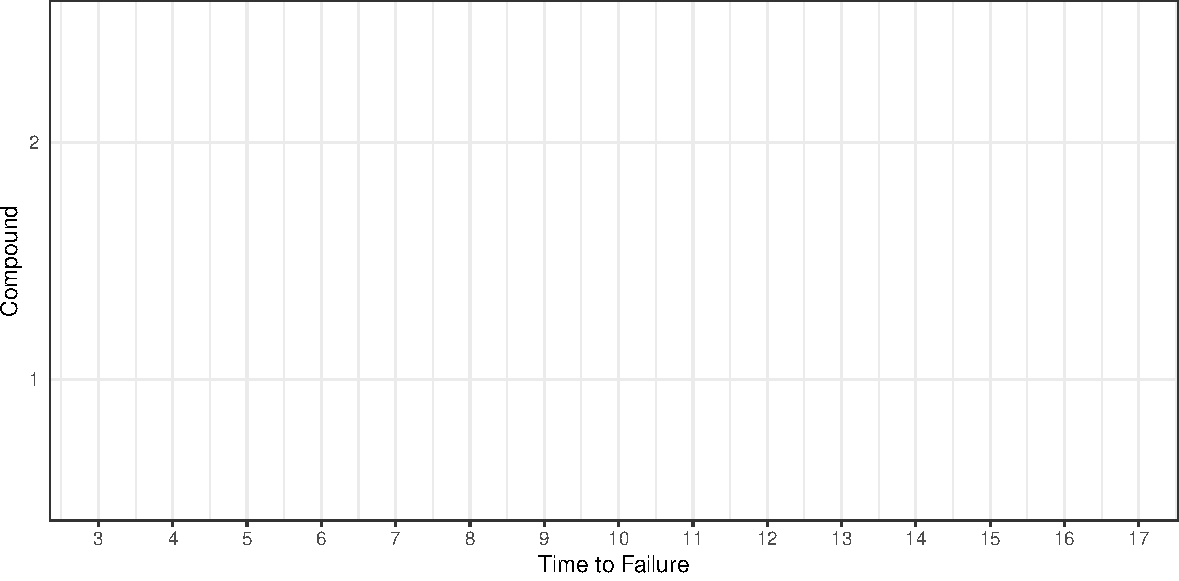
\includegraphics[width=.9\linewidth]{stat305-exam3_files/figure-latex/unnamed-chunk-2-1}
\pagebreak

\question

The quality of a diamond is often described in terms of the four C's: -
carat (the diamonds mass, with 1 carat = 200 milligrams), - cut (a
description of how well the diamond has been shaped), - color (the less
color the more rare), - clarity (a description of the flaws in the
diamond). Of these, carat is the most easily understood in terms of its
impact on the diamonds value: all things being equal, the larger the
diamond the higher its value.

The following plot shows the sale price of 375 diamonds (in thousands of
dollars), which were appraised by experts as having an ideal cut,
internally flawless clarity, and being colorless or essentially
colorless.

\begin{figure}[h]

{\centering 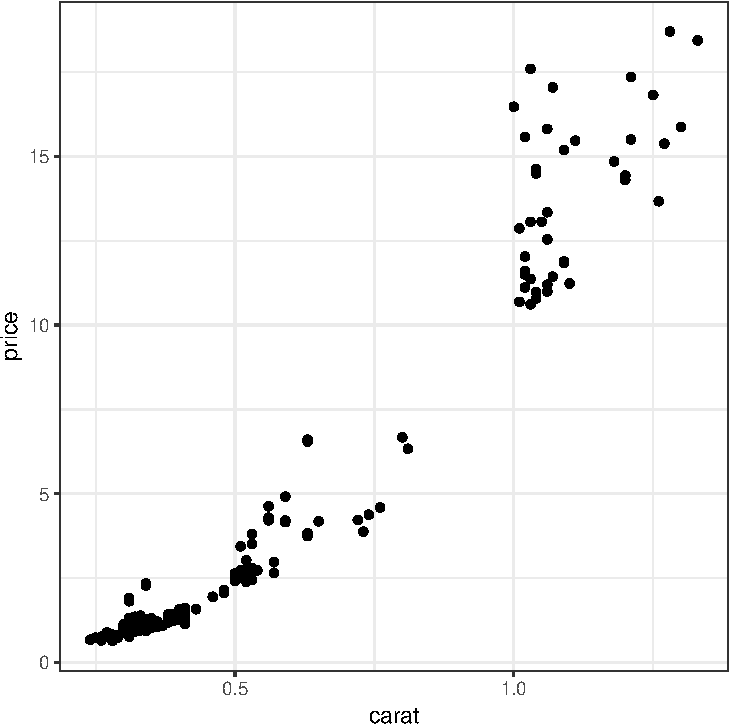
\includegraphics[width=.5\linewidth]{stat305-exam3_files/figure-latex/unnamed-chunk-4-1} 

}

\caption{Plot depicting the sale price of 375 diamonds with the same quality of cut, clarity, and color. There is a general pattern indicating that higher carat (i.e., the mass) is associated with higher price.}\label{fig:unnamed-chunk-4}
\end{figure}

Here are some summaries of the data (using carat as the \(x\)-value and
price as the \(y\)-value):

\[\sum_{i=1}^{375} x_i = 163.68 \hspace{3cm} \sum_{i=1}^{375} x_i^2 = 94.6962\]

\[\sum_{i=1}^{375} y_i = 1018.531 \hspace{3cm} \sum_{i=1}^{375} y_i^2 = 8802.953653\]

\[\sum_{i=1}^{375} x_i y_i = 808.54225\]

\newpage

The following parts are based on using a linear relationship between
carat (\(x\)) and price (\(y\)). \qparts{
\part[5] Using the above summaries, write the equation of the fitted linear relationship between carat and price. \vspace{3cm}
\part[3] Using the fitted line, what do we suppose the price would be for a 1.07 carat diamond? \vspace{3cm}
\part[3] The actual price of a 1.07 carat diamond in the data is 11.434 thousand dollars. What is the residual for this specific diamond using the linear model? \vspace{3cm}
\part[3] For the linear relationship, find \(r\), the sample correlation coeffecient and \(R^2\), the coeffecient of determination. \vspace{3cm}
\part[3] Explain whether or not the fitted line did a good job describing the relationship between carat and price. \vspace{3cm}
} \newpage A better fit may be found using a quadratic model, where
price depends on carat and \(\text{carat}^2\). The JMP output below
comes from fitting a this quadratic relationship using price as the
response (\verb!price!) and carat (\verb!carat!) and \(\text{carat}^2\)
(\verb!carat_sq!) as the model variables.

\centerline{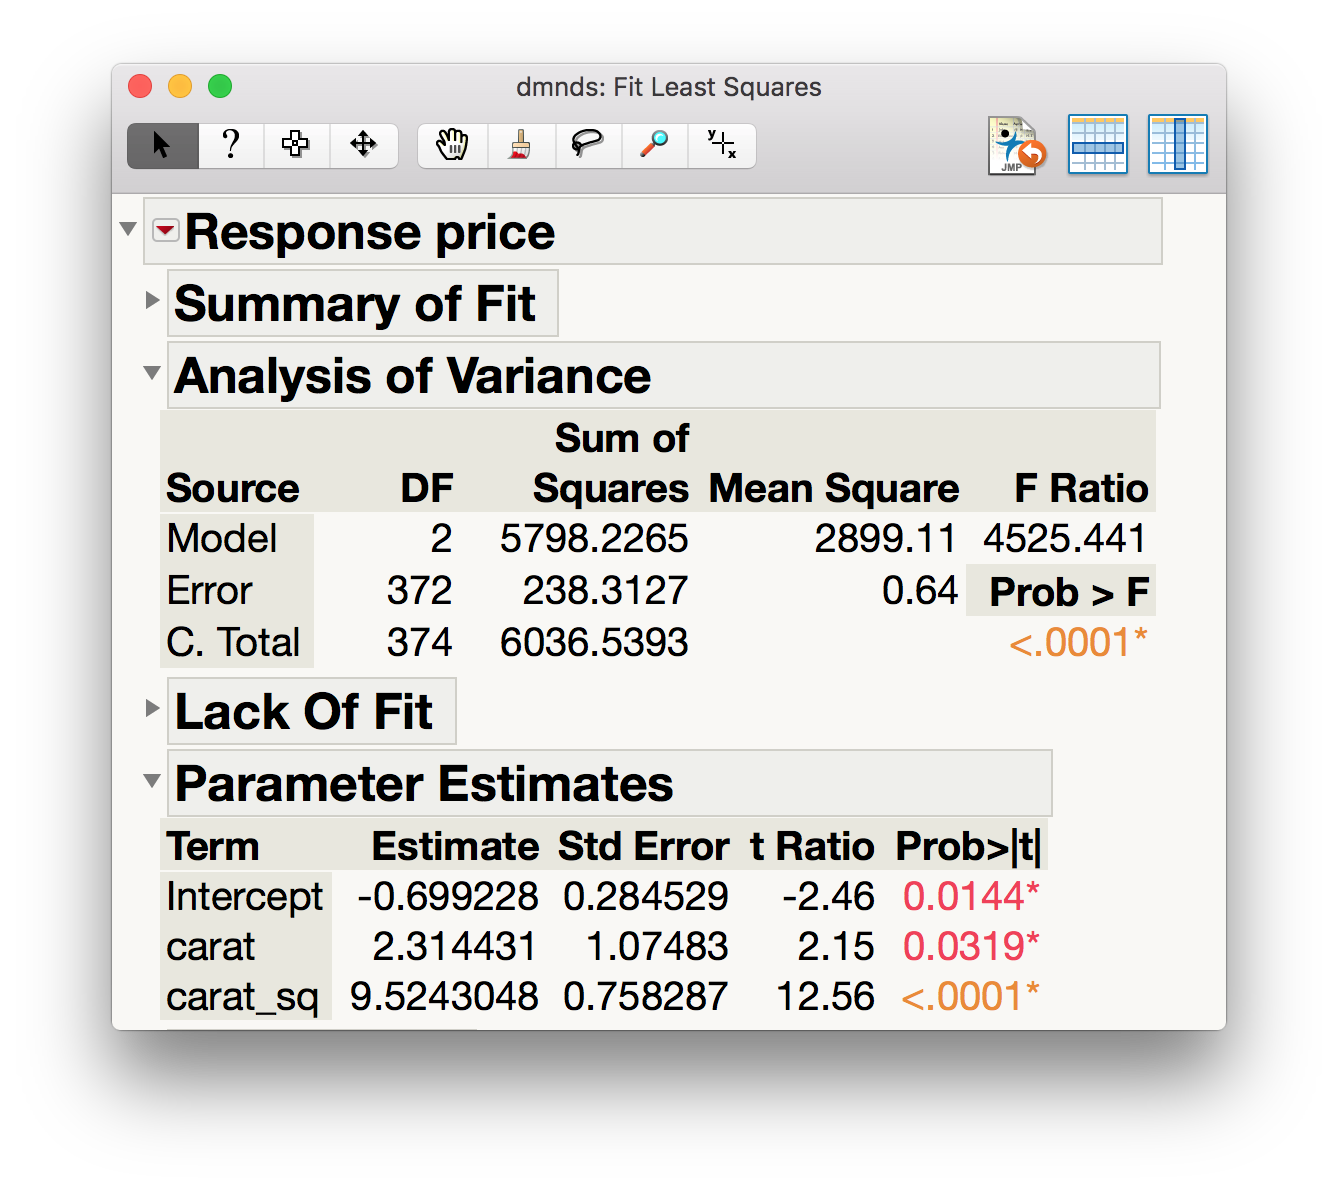
\includegraphics[scale=.35]{carat_sq_fit}}
\qparts{
\part[5] Write the equation of the fitted quadratic relationship. \vspace{2cm}
\part[3] Using the fitted quadratic relationship, what do we suppose the price would be for a 1.07 carat diamond? \vspace{2cm}
\part[3] The actual price of a 1.07 carat diamond in the data is 11.434 thousand dollars. What is the residual for this specific diamond using the quadratic model? \vspace{2cm}
\part[3] Find the value of \(R^2\) for the fitted quadratic relationship. \vspace{2cm}
\part[3] Does it appear that a quadratic relationship is better than the linear relationship? \vspace{2cm}
}

\newpage

\question

Let \(X\) be a normal random variable with a mean of 5 and a varaince of
4 (i.e., \(X \sim N(5,4)\)) and let \(Z\) be a random variable following
a standard normal distribution. Find the following probabilities (note:
the attached standard normal probability table may be helpful): \qparts{
   \part[2] $P(Z \le 1.5)$ \vspace{2cm}
   \part[2] $P(|Z| \ge 1.25)$ \vspace{2cm}
   \part[2] $P(1 \le X < 9)$ \vspace{2cm}
   \part[2] $P(|X| \le 5)$ \vspace{2cm}
}

\question

Suppose that \(X\) is a continuous random variable with probability
density function (pdf):
\[f(x) = \begin{cases} 0 &  x < 0 \\ 2 e^{-2x} &  x \ge 0 \end{cases}\]

\qparts{
 \part[3] Find F(x), the cumulative probability function. \vspace{3cm}
 \part[3] What is the probability that $X$ takes a value less than 1? \vspace{2cm}
 \part[3] What is the probability that $X$ takes a value greater than 2? \vspace{2cm}
}

\newpage

\question

Consider the following scenario:

A fair die is rolled and the number of dots facing up is counted. For
each dot facing up on the die, a fair coin is flipped and the number of
times the coin lands heads up is recorded.

\begin{itemize}
   \item let $N$ be the number of dots facing up from the roll of the die
   \item let $X$ be the number of heads resulting from the flips of the coin.
\end{itemize}

For the outcome where we roll a 5, then \(N = 5\) and we will toss the
coin 5 times. Using the number of times we flip heads as our outcome of
interest, we will have the conditional distribution of \(X | N = 5\) to
be binomial(5, \(0.5\)). More generally, we can write:
\[f_{X|N}(x|n) = \frac{n!}{(n - x)! x!} (0.5)^x (0.5)^{n - x}, x = 0, 1, ..., n\]
and 0 otherwise.

\qparts{
\part[3] Find the marginal probability function for $N$, $f_N(n)$. \vspace{2cm}
\part[3] Find the conditional probability that $X = 2$ given that $N = 4$, $f_{X|N}(2|4)$. \vspace{2cm}
\part[3] Find the joint probability $f_{NX}(4,2)$. \vspace{2cm}
\part[3] Find the joint probability $f_{NX}(3,2)$. \vspace{2cm}
\part[3] Find $f_{X}(2)$. \vspace{2cm}
\part[4] Find the probability that we rolled a 4 given that we had two heads from our coin flips, $f_{N|X}(4|2)$. \vspace{2cm}
}

\newpage

\question

An inspector examining the dependability of a certain gas pump fills 50
containers until the pump reads 1.00 gallons. If the pump is completely
accurate, then each container should have 1.00 gallons of gasoline.
However, since nothing is completely consistent, there will be
differences from one container to the next.

Suppose that it is known that the true standard deviation of the amount
of gasoline the pump recognizes as 1.00 gallons is \(\sigma = 0.2\)
gallons.

The average of the 50 gallon samples is \(\bar{x} = 0.992\) gallons

The following table may be useful:

\begin{table}[h]
   \centering
   \caption{z's for use in Two-sided Large-$n$ intervals for the mean}
   \begin{tabular}{cc}
      \hline \\
      Desired Confidence & $z$ \\
      \hline 
      80\% & 1.28 \\
      90\% & 1.645 \\
      95\% & 1.96 \\
      98\% & 2.33 \\
      99\% & 2.58 \\
      \hline 
   \end{tabular}
\end{table}

\qparts{
\part[4] Provide a 90\% confidence interval for the mean volume of gasoline recognized by the pump to be 1.00 gallons. \vspace{2cm}
\part[4] Provide a 95\% confidence interval for the mean volume of gasoline recognized by the pump to be 1.00 gallons. \vspace{2cm}
\part[4] Provide a 99\% confidence interval for the mean volume of gasoline recognized by the pump to be 1.00 gallons. \vspace{2cm}
\part[4] Interpret these confidence intervals - is there evidence that the meter on the pump is not accurate? 
}

\newpage

\question A group of scientists are trying to understand the effects of
temperature on two O-ring designs for a rocket. By placing the O-ring
(attached to a valve) in a chamber and slowly lowering the chamber's
temperature, the scientists are able to record the temperature at which
the O-ring fails by monitoring when the valve begins to leak. After
testing 10 O-rings for each type, the scientists find the mean failure
temperature for the first O-ring design sample to be \(50\) K with a
sample variance of 10 and the mean failure temperature of the second
O-ring sample to be \(53\) K with a sample variance of \(20\). \qparts{
\part[4] Provide a 95\% confidence interval for the true failure temperature of the first O-ring design. \vspace{3cm}
\part[4] Provide a 95\% confidence interval for the true failure temperature of the second O-ring design. \vspace{3cm}
\part[6] Assume that the failure temperatures for both O-ring designs is normally distributed. Provide a 95\% confidence interval for difference in the two designs. \vspace{3cm}
\part[2] Is there any clear evidence that one of the O-ring designs will survive at lower temperatures than the other? Explain why or why not.
}

\newpage

\question

An arctic research station recently did a major overhaul to their server
system hardware and the technicians are checking to make sure that there
has been no loss in download speed. The previous download speed had an
average of 63.4 Mbps. A systems analyst took 10 readings on the download
speeds during the course of a day to check. Her results are below (in
Mbps):

\begin{center} 63.1, 62.89, 62.76, 62.77, 63.23, 63, 63.11, 62.74, 62.98, 62.95 \end{center}

The sample average is 62.95 and the sample variance is 0.027.

\qparts{
\part[5] Provide a 90\% confidence interval for the mean download speed. \vspace{2cm}
\part[5] Provide a 95\% lower confidence bound for the mean download speed. \vspace{2cm}
\part[10] Conduct a hypothesis test at the 95\% confidence level for the null hypothesis $\mu \ge 63.4$ against the alternative $\mu < 63.4$. Include your hypothesis statement, the choice of test statistic, the p-value, and your conclusion.
}

\end{questions}

\end{document}
